\documentclass[12pt,a4paper,final,titlepage,openany]{report}

\usepackage[utf8]{inputenc}
\usepackage{amsmath}
\usepackage{amsfonts}
\usepackage{amssymb}
\usepackage{makeidx}
\usepackage{graphicx}
\usepackage{layout}
\usepackage{lscape}
\usepackage{xfrac}
\usepackage{tabularx}
\usepackage{rotating}
\usepackage{longtable}
%\usepackage{todonotes}

\usepackage{hyperref}
\hypersetup{
  colorlinks=true,
  linktoc=all,
  citecolor=black,
  linkcolor=black,
  urlcolor=red,
  % linktocpage=true,
}
\usepackage{cleveref}

\usepackage[square,numbers,sort&compress, sectionbib]{natbib}
\usepackage{chapterbib}

\setlength\bibhang{.3in}

\usepackage{tocloft} % for table of contents

\usepackage{lineno}
\usepackage{setspace}
\onehalfspacing
\usepackage{microtype}
\usepackage{color}
\usepackage{fancyhdr}
\usepackage[labelfont=bf]{caption}
% For electronic submission use:
\usepackage[inner=2cm,outer=2cm,top=2cm=bottom=2cm]{geometry}
% For printing use:
%\usepackage[inner=4cm,outer=2cm,top=2cm=bottom=2cm]{geometry}
\usepackage{tocbibind}

\usepackage{subfig}    % needed for \subfloat
\usepackage{titlesec}
\usepackage{derivative}
\usepackage{enumerate} % needed for the enumerate environment

\usepackage{subfiles} % Best loaded last in the preamble

%glossary for acronyms
\usepackage[acronym,nonumberlist,toc,section=subsection,numberedsection=nolabel]{glossaries}
\newacronym{QiML}{QiML}{Quantum-Inspired Machine Learning}
\newacronym{QML}{QML}{Quantum Machine Learning}
\newacronym{QNN}{QNN}{Quantum Neural Network}
\newacronym{VQC}{VQC}{variational quantum circuit}
\newacronym{QAOA}{QAOA}{Quantum Approximate Optimization Algorithm}

\newacronym{BERT}{BERT}{Bidirectional Encoder Representations from Transformers}
\newacronym{GPT}{GPT}{Generative Pre-trained Transformer}

\newacronym{AUC}{AUC}{area under the curve}


\setlength{\headheight}{14.5pt}
\addtolength{\topmargin}{-2.5pt}

\fancyhf{}
\fancyhead[L]{\bfseries\nouppercase{\leftmark\hfill\rightmark}}
\fancyfoot[C]{\thepage}
\pagestyle{fancy}

\newcommand\frontmatter{\pagenumbering{roman}}
\newcommand\mainmatter{\cleardoublepage\pagenumbering{arabic}}


\begin{document}
\begin{titlepage}
  %\newgeometry{left=20mm,right=20mm,top=2.5cm,bottom=2cm}

  \thispagestyle{empty}
  \vspace*{\fill}

  \begin{center}

    \begin{center}
      
\includegraphics[width=0.25\linewidth]{img/uwa.PNG}
    \end{center}

    \vspace{1cm}
    {\scshape\LARGE University of Western Australia \par}
    \vspace{1.25cm}
    {\scshape\Large Data Science Research Project\par}
    \vspace{1.5cm}

    {\Large\bfseries Quantum Transformers: \\
    From Circuit Design to Performance Comparison\par}

    \vspace{1.5cm}
    {\Large\itshape Wei Chun Nicholas Choong\par}
    \vspace{1.25cm}

    \vspace{1.5cm}
    Supervised by\par
    Assoc.~Prof.~Wei Liu \par
    Assoc.~Prof.~Du Huynh \par
    Prof.~Jingbo Wang \par
    Prof.~Fredrick Cadet \par
    \vspace{1.5cm}
    \large October 2024\par

  \end{center}

  \vspace*{\fill}
  \clearpage
  \restoregeometry
\end{titlepage}


\restoregeometry
\sloppy
\frontmatter

\chapter*{Abstract}
\label{chap:abstract}
\addcontentsline{toc}{chapter}{Abstract}
This dissertation investigates the integration of quantum variational
circuits (VQCs) into transformer models to explore the potential
advantages of quantum computing in natural language processing (NLP)
tasks. By incorporating both basic and strong VQCs, along with
encoding methods such as amplitude and angle encoding, we compare the
performance of quantum transformers to classical transformers.
Extensive experiments were conducted using datasets like IMDb,
Amazon, and Yelp to evaluate models with and without embedding
layers. The results show that quantum models, particularly those
using amplitude encoding, can outperform classical models in certain
configurations, achieving superior accuracy. Additionally, we have
successfully reduced the training time by leveraging efficient
quantum computing frameworks. This work
demonstrates the viability of quantum machine learning
models and provides insights into their potential applications in
complex NLP tasks. The study also discusses future directions for
improving quantum transformer architectures, including further
optimisations in encoding strategies and circuit designs.


\pagebreak

\setcounter{tocdepth}{2}
\tableofcontents
\pagebreak
\listoffigures
\pagebreak
\listoftables

\mainmatter
\raggedbottom

\chapter{Introduction}
\label{chap:introduction}
\section{Motivations}
\label{sec:motivations}
Over the past few decades, the exponential growth of deep learning
has led to groundbreaking advancements that have not only transformed
computer science but have also permeated numerous other disciplines
and industries. The profound impact of deep learning is evident in
its integration into various aspects of daily life—from enhancing
virtual assistants and powering autonomous vehicles to
revolutionising healthcare diagnostics and financial analytics. Deep
learning models have achieved superhuman performance in tasks such as
computer vision, natural language processing (NLP), and generative
artificial intelligence (AI), enabling the creation of human-like
outputs across multiple media, including text, images, audio, and video.

This influence was further emphasised in 2024 when John J. Hopfield
and Geoffrey E. Hinton were jointly awarded the Nobel Prize in
Physics for their seminal contributions to artificial neural
networks. Hopfield's pioneering work on associative memory models and
Hinton's revolutionisation of the backpropagation algorithm laid the
foundational architectures of modern deep learning. The recognition
by the Nobel Committee not only highlights the interdisciplinary
nature of their work but also cements the significance of deep
learning in advancing scientific and technological progress.

Despite these remarkable achievements, the rapid evolution of deep
learning has brought several limitations to the forefront,
particularly concerning the computational and financial resources
required to train increasingly complex models. As model architectures
grow in depth and breadth, the demand for vast amounts of data and
processing power escalates, presenting significant barriers to
scalability and broader application. Classical hardware, while
powerful, faces inherent limitations in handling the ever-growing
demands of cutting-edge AI models. This is especially evident in
emerging fields like multimodal learning, artificial general
intelligence, and protein folding, where the sheer scale of
computations challenges even the most advanced classical systems.

In response to these challenges, quantum computing has emerged as a
promising paradigm that could potentially overcome the limitations of
classical computing. By leveraging the principles of quantum
mechanics, quantum computing offers the potential to process
information in fundamentally new ways, providing exponential speedups
for certain tasks. Quantum phenomena such as superposition and
entanglement allow quantum computers to explore vast computational
spaces more efficiently than classical bits, opening up new avenues
for tackling problems previously considered intractable. The
implications of quantum computing extend across various sectors,
including cryptography, optimisation, and artificial intelligence.

At the intersection of deep learning and quantum computing lies the
potential for a new class of models: quantum deep learning models,
particularly quantum transformers. Inspired by classical transformer
models—which have revolutionised NLP, computer vision, and generative
AI—these quantum counterparts aim to enhance capabilities by
exploiting the unique properties of qubits, such as superposition,
entanglement, and quantum parallelism. Quantum transformers hold the
promise of processing information more efficiently, enabling more
scalable and resource-efficient models. This presents exciting
possibilities for advancing tasks like language translation, image
generation, and even more complex applications that push the boundaries of AI.

Recent developments have seen claims that quantum transformers can
outperform classical models in specific scenarios, achieving
comparable or superior results with fewer resources. For instance,
the work of~\citet{Cherrat_2024} suggests that quantum vision
transformers can attain accuracies that meet or exceed those of
classical vision transformers. However, these claims face significant
challenges. Quantum hardware remains in developmental stages, making
the implementation of quantum algorithms complex and
resource-intensive. Additionally, training quantum neural networks,
including quantum transformers, often encounters the problem of
barren plateaus—regions in the optimisation landscape where gradients
vanish, hindering effective training.

Moreover, the theoretical and practical aspects of integrating
quantum computing with deep learning are still under active research.
Issues such as error correction in quantum systems, decoherence, and
the scalability of quantum circuits pose substantial hurdles. The
quantum machine learning community is actively exploring algorithms
and architectures that can mitigate these problems, aiming to unlock
the full potential of quantum-enhanced AI.

The convergence of quantum computing and deep learning represents a
frontier with immense potential but also significant uncertainty. As
both fields continue to evolve, their intersection could lead to
breakthroughs that redefine computational capabilities and transform
industries. Understanding the current landscape, the challenges, and
the opportunities is crucial for advancing this emerging area of research.

The integration of quantum mechanics into deep learning models also
raises philosophical and ethical considerations. The prospect of
machines that can process information in fundamentally new ways
prompts questions about the future of AI, the nature of intelligence,
and the potential societal impacts. There is a growing discourse on
how quantum-enhanced AI could influence areas such as data privacy,
security, and employment, highlighting the need for interdisciplinary
collaboration in addressing these concerns.

Historically, technological advancements have often led to paradigm
shifts in society. The steam engine ignited the Industrial
Revolution, electricity transformed daily life and industry, and the
internet revolutionised communication and information access.
Similarly, the fusion of quantum computing and AI could bring forth a new
era of innovation. Industries such as pharmaceuticals might see
accelerated drug discovery processes, finance could benefit from more
sophisticated modeling and risk assessment, and logistics could
achieve unprecedented optimisation levels.

In summary, the advent of quantum computing offers a promising avenue
to address the limitations faced by classical deep learning models.
Quantum transformers, by harnessing the unique properties of quantum
mechanics, could potentially revolutionise AI by enabling more
efficient and powerful models. As we stand at the cusp of this new
era, exploring the interplay between quantum computing and deep
learning is not only intriguing but also essential for the future of
computational science.

The journey toward realising the full potential of quantum
transformers is fraught with challenges but also rich with
opportunities. Continued research and innovation in this field could
lead to significant breakthroughs that redefine the limits of machine
learning and computation. The implications of such advancements are
vast, promising transformative applications across industries and
disciplines, and ushering in a new chapter in the story of
technological progress.

\section{Research Objectives}
\label{sec:research_objectives}

The convergence of quantum computing and deep learning presents a
frontier ripe with potential for significant advancements in
artificial intelligence. This research seeks to explore this
intersection by focusing on quantum transformers.
The primary objectives of this study are outlined as follows:

\begin{enumerate}
  \item  \textbf{Design and Optimise New Quantum Circuits}

    The goal is to explore and implement various quantum circuit
    designs for use in quantum transformers. This includes
    investigating different data encoding methods such as amplitude
    encoding, angle encoding, and block encoding to effectively
    represent input data within quantum circuits. We will employ
    Pennylane's basic and strong entangling layers for constructing
    \glspl{VQC} to enhance the expressibility
    and entangling capabilities of the quantum circuits.
    Additionally, we will use an autoencoder to adjust the dimension
    of the word embedding to fit into the next layer, ensuring
    efficient data flow through the quantum and classical components.

  \item  \textbf{Compare Quantum and Classical Models and Attempt to
    Reproduce Existing Results}

    To conduct a thorough comparison between quantum and classical
    transformer models, focusing on accuracy, \gls{AUC}, and computational
    resources. This includes an effort to reproduce results from
    recent studies to assess the performance and potential benefits
    of quantum circuits in these models.

  \item  \textbf{Reduce Quantum Model Training Time on Simulated
    Quantum Computers}

    To explore different quantum computing frameworks, such as
    Pennylane and TensorCircuit, as well as classical deep learning
    frameworks like PyTorch and TensorFlow. The goal is to optimise
    the training process, making quantum transformer models more
    manageable to be trained on simulated quantum computers,
    potentially reducing the overall training time and making them
    more feasible for practical applications.

\end{enumerate}

By pursuing these objectives, our research aims to contribute to the
foundational understanding and practical advancement of quantum
transformers. This work seeks to explore and demonstrate the
capabilities and limitations of integrating quantum computing with
deep learning, ultimately contributing to the evolution of artificial
intelligence in the quantum era.

\section{Our Contributions}
\label{sec:contributions}

TODO: This research makes several key contributions to the field of quantum...

\subsection{Open Source Code Contributions}
\label{subsec:open_source_code_contributions}

As part of this research, we have contributed to the
open-source community by making our code publicly available. The code
for the quantum transformers, including the design and implementation
of quantum circuits, is hosted on \href{https://github.com/}{GitHub}.
This repository provides a
comprehensive set of tools and resources for researcherss interested
in quantum machine learning and transformer-based models. Our code
repository can be found at
\url{https://github.com/NicholasChoong/QuantumTransformer}.

\section{Outline}
\label{sec:outline}

This dissertation is structured as follows:

\begin{enumerate}
  \item \textbf{\hyperref[chap:literature]{Chapter 2: Literature Review}}

    This chapter presents a comprehensive review of the existing
    literature on transformer models, quantum machine learning,
    quantum neural networks, and variational quantum circuits. It
    also discusses various data embedding techniques and the
    limitations of current models, providing a foundation for the
    development of quantum transformers.

  \item \textbf{\hyperref[chap:methodology]{Chapter 3: Methodology}}

    The methodology outlines the research design, data collection,
    and the detailed implementation of both classical and quantum
    transformers. The approaches for training and evaluating these
    models are also described.

  \item \textbf{\hyperref[chap:results]{Chapter 4: Experiments and Results}}

    This chapter details the experimental setup, describes the
    conducted experiments, and presents the results of the quantum
    and classical transformer models. The performance metrics and
    analysis of the models are also discussed in this section.

  \item \textbf{\hyperref[chap:conclusion]{Chapter 5: Conclusion and
    Future Work}}

    The conclusion summarises the key contributions of this research,
    reflecting on the outcomes of the experiments and the broader
    implications for the field of quantum machine learning. The
    chapter also outlines potential directions for future research.

  \item \textbf{\hyperref[apx:proposal]{Appendices}}

    The appendices include supplementary materials such as the
    research proposal, pseudo code, and a detailed analysis of the
    training speed of the models.
\end{enumerate}


\chapter{Literature Review}
\label{chap:literature}
\section{Background}
\label{sec:background}

\subsection{Transformer Models}
\label{subsec:transformer_models}
Transformer architectures have emerged as a dominant paradigm in
natural language processing. Unlike traditional recurrent neural
networks and convolutional neural networks, transformers avoid
sequential processing in favour of self-attention mechanisms that
allow for parallel processing of input sequences.

The key innovation of transformers lies in their ability to capture
long-range dependencies within input sequences, making them
particularly effective for tasks such as language translation, text
generation, and sentiment analysis. Models such as \gls{BERT} and
\gls{GPT} have achieved state-of-the-art performance on various
natural language processing benchmarks,
demonstrating the power of transformer architectures.

\subsection{Quantum-Inspired Machine Learning}
\label{subsec:quantum_inspired_machine_learning}

\gls{QiML} refers to a class of machine learning algorithms that draw
inspiration from quantum mechanics but are implemented on classical
hardware. Unlike \gls{QML}, which relies on quantum computation to
process data, \gls{QiML} applies quantum principles to classical
algorithms without the need for quantum devices. \gls{QiML} has
gained attention due to its potential to harness computational
advantages by simulating quantum effects through classical
frameworks. Techniques such as tensor networks, dequantized
algorithms, and quantum-inspired optimisation algorithms are
prominent examples of \gls{QiML} approaches. These methods have been
shown to improve efficiency and performance on certain tasks
traditionally solved using classical machine learning models.

The relationship between \gls{QiML} and \gls{QML} can be understood
as a spectrum of quantum mechanics integration, as illustrated in
Figure~\ref{fig:qiml_levels}. On the left side of the spectrum, we
have classical approaches
like dequantized algorithms that employ quantum-inspired techniques
but operate entirely within classical systems. As we move to the
right, more quantum mechanics are integrated, including tensor
networks and density matrices used as features, which bridge
classical and quantum methods. Finally, on the far right, we
encounter true \gls{QML} approaches, such as \glspl{VQC} and
quantum kernels, which require quantum hardware
for computation.

\begin{figure}[ht] \centering
  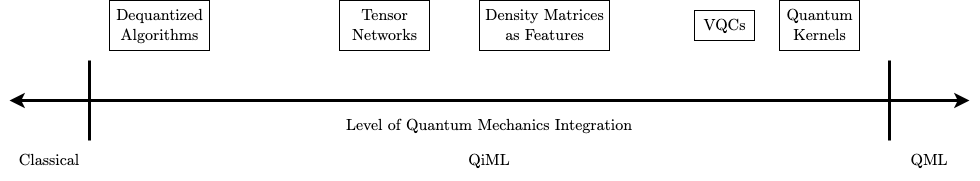
\includegraphics[width=\textwidth]{img/qiml_levels.png}
  \caption{A spectrum of machine learning approaches from classical to
    quantum-inspired to quantum-based
  methods~\cite{huynh2023quantuminspiredmachinelearningsurvey}.}
  \label{fig:qiml_levels}
\end{figure}

The primary difference between \gls{QML} and \gls{QiML} lies in their
reliance on quantum hardware. While \gls{QML} explores the use of
quantum computers to solve machine learning problems, \gls{QiML}
remains entirely within the classical computational realm, applying
quantum concepts without leveraging quantum hardware. This
distinction makes \gls{QiML} more accessible given current
technological limitations in quantum computing.

It is important to note that our research focuses on \gls{QML}, not
\gls{QiML}. In this project, we will directly employ simulated
quantum hardware and algorithms to explore how quantum computing can
enhance machine learning, specifically for sentiment analysis tasks
using transformer models.

\subsection{Quantum Neural Network}
\label{subsec:quantum_neural_network}
A \gls{QNN} is a machine learning architecture that
employs quantum computing principles. It has a set of trainable
parameters (\(\theta\)) that can be realised based on an initial
probability distribution. The goal of machine learning is to train
these parameters and achieve a probability distribution that closely
resembles the underlying problem. A model with high generalisation
ability can identify existing patterns in the testing data without
overfitting to the training data.

The specific approach involves providing the data to the quantum
model through a process called a data embedding strategy, which can
significantly impact the functional representation of the model. The
objective function is the expectation value of a variational
quantum circuit. These circuits make use of continuous variable group
rotations, allowing for the manipulation of quantum states.

Since there is no established framework for designing variational
quantum circuits, it is crucial to fine-tune the circuit
architecture, as it can directly affect the performance of the
quantum neural network model. Fortunately, many quantum computing
libraries, such as Pennylane and Qiskit, provide templates for
\glspl{VQC}.

\subsection{Data Embedding}
\label{subsec:data_embedding}
There are many encoding strategies for loading classical data into a
quantum computer but for this literature, we will only be discussing
about three encoding strategies. They are Angle embedding, Amplitude
embedding, Quantum Approximate Optimization Algorithm (QAOA)
embedding and Block Encoding.

\begin{itemize}
    % \setlength{\itemsep}{-1ex}
  \item Angle embedding~\cite{schuld2021supervised} is a
    straightforward strategy where classical data features are
    encoded into the angles of quantum gates. Each feature is mapped
    to the rotation angle of a qubit, typically using single-qubit
    rotation gates such as RX, RY, or RZ. To encode \(n\) features,
    Angle embedding requires \(n\) qubits, as each feature is
    directly assigned to a qubit's rotation. While this encoding
    method is straightforward, it can be resource-intensive for large
    datasets, as the number of qubits required grows rapidly with the
    number of features.

  \item Amplitude embedding~\cite{schuld2021supervised} is a more
    complex strategy that encodes classical data into the amplitudes
    of a quantum state. This method involves preparing a quantum
    state where the amplitudes of the state vector represent the
    classical data values. Given a classical data vector \( x = [x_1,
    x_2, \dots, x_n] \), the first step is to normalise the data. The
    normalisation is done by dividing each element by the Euclidean
    norm \( \|x\| \), where:

    \begin{equation}
      \| x \| = \sqrt{x_1^2 + x_2^2 + \dots + x_n^2}
    \end{equation}

    This ensures the total probability of the quantum state is 1. The
    normalised vector is:

    \begin{equation}
      \tilde{x} = \frac{1}{\| x \|} [x_1, x_2, \dots, x_n]
    \end{equation}

    Next, the normalised vector \( \tilde{x} \) is encoded into the
    amplitudes of a quantum state \( |\psi \rangle \), which can be
    represented as:

    \begin{equation}
      |\psi \rangle = \sum_{i=1}^{n} \tilde{x}_i |i\rangle
    \end{equation}

    where \( |i\rangle \) are the computational basis states. To
    encode \( n \) features, \( \log_2(n) \) qubits are required,
    assuming \( n \) is a power of two, because the quantum state
    must accommodate all \( n \) amplitudes, and \( \log_2(n) \)
    qubits are needed to create a state with \( n \) possible
    amplitudes. For example, if \( n = 4 \), the resulting quantum
    state would be:

    \begin{equation}
      |\psi \rangle = \tilde{x}_1 |00\rangle + \tilde{x}_2 |01\rangle
      + \tilde{x}_3 |10\rangle + \tilde{x}_4 |11\rangle
    \end{equation}

    This encoding strategy is particularly useful for applications
    that involve processing high-dimensional data, as it can
    significantly reduce the number of qubits required compared to
    other encoding methods.
  \item The Quantum Approximate Optimization Algorithm (QAOA)
    embedding~\cite{lloyd2020quantum} is a hybrid approach that
    encodes classical data into the parameters of a QAOA circuit.
    QAOA is originally designed for solving combinatorial
    optimisation problems but can be adapted for data encoding by
    associating the problem parameters with data features. The number
    of qubits required for QAOA embedding depends on the specific
    problem and the depth of the QAOA circuit but generally requires
    at least as many qubits as there are features to encode the data
    adequately. For \(n\) features, a minimum of \(n\) qubits is
    typically needed, with additional qubits possibly required
    depending on the circuit's complexity and the problem structure.
    In general, QAOA embedding requires several qubits that scale
    with the number of variables and constraints in the optimisation
    problem. This encoding strategy is particularly useful for
    solving combinatorial optimisation problems on quantum computers.
  \item Block encoding embeds a non-unitary operator as a sub-block
    of a larger unitary matrix,
    allowing non-unitary matrices to be processed within quantum circuits.
    In general, a matrix \( A \in \mathbb{C}^{N \times N} \), where
    \( N = 2^n \), can be block-encoded into a unitary matrix by
    extending the dimension of the matrix and adding ancilla qubits.

    The block-encoded matrix \( U \) can be represented as:
    \begin{equation}
      U =
      \begin{pmatrix}
        A & * \\
        * & *
      \end{pmatrix}
    \end{equation}

    The block-encoded form allows us to work with non-unitary
    operators in a quantum framework while maintaining the overall
    unitary evolution required by quantum mechanics.
    To perform block encoding, we use a combination of quantum
    oracles \( U_A \) and \( U_B \). The oracle \( U_A \) encodes the
    matrix elements \( A_{i,j} \) into the amplitude of an ancillary
    qubit, while \( U_B \) ensures proper indexing over the matrix
    entries. The combination of these operations allows the matrix \(
    A \) to be embedded as a block within a larger unitary matrix.
    This technique is particularly useful for quantum algorithms that
    involve manipulating large, structured, or sparse matrices, as it
    efficiently encodes the matrix into a quantum state without
    directly applying non-unitary operations. Block encoding is
    crucial for several quantum machine learning and linear algebra
    algorithms, enabling the practical implementation of otherwise
    challenging quantum computations.
\end{itemize}

\subsection{Variational Quantum Circuit}
\label{subsec:variational_quantum_circuit}
In classical neural networks, increasing the number of parameters
enhances the expressivity of the models. However, in quantum
circuits, having too many parameters can lead to redundancy because
over-parameterised circuits may not improve performance and can make
optimisation more challenging. Excess parameters can result in
entangled states that do not contribute meaningfully to the solution,
potentially causing the circuit to explore a larger, less relevant
portion of the parameter space. As mentioned earlier, there are no
standard frameworks for designing these architectures, resulting in
varying designs from one author to another. Nonetheless, quantum
computing libraries offer templates for \glspl{VQC} to facilitate their use.

\begin{equation}
  U(\theta) = \prod_{i=1}^{L} U_{i}(\theta_i)
\end{equation}

where \(L\) is the number of \gls{VQC}
iterations, \(U\) is the \gls{VQC} unitary,
\(\theta=(\theta_1,...,\theta_L )\) is a set of trainable parameters.

The \acrlong{VQC}~\cite{li2023quantum} consists of
repeated rotation gates applied to each qubit, along with CNOT gates
that entangle the qubits to form a highly entangled system. These
rotation gates, such as RX, RY, or RZ, adjust the qubit states based
on the trainable parameters. The CNOT gates, on the other hand,
create entanglement between pairs of qubits, enabling complex
interactions across the entire quantum system.

This combination of rotation and entangling gates allows the circuit
to explore a wide range of quantum states, enhancing its ability to
model complex functions and relationships within the data. By
fine-tuning the parameters of these gates, the quantum circuit can be
optimised to solve specific problems or recognise patterns in data.
However, designing these circuits requires careful consideration, as
the arrangement and number of gates can significantly impact the
circuit's performance and computational efficiency.

\subsection{Gradient Calculation}
\label{subsec:gradient_calculation}
The most common gradient calculation method in classical machine
learning is the back-propagation algorithm. This technique computes
the gradient of each function that the trainable parameters pass
through, using the chain rule to create an automatically
differentiable machine learning routine. In the context of quantum
machine learning, back-propagation can also be employed. However,
there’s a key difference: it requires access to the quantum state
vector. As a result, its application is limited to quantum simulators
rather than real quantum processing units (QPUs).

As a result, it is crucial to find alternative methods that can
operate on actual QPUs. One such alternative is the finite difference
method~\cite{Schuld_2019}, a form of numerical differentiation used
to approximate derivatives. The finite difference method estimates
the derivative of a function by evaluating the function at slightly
shifted parameter values and calculating the ratio of the change in
the function value to the change in the parameter.

However, while finite difference provides a useful approximation, it
can be quite unstable when used iteratively in processes such as
gradient descent. This instability arises because the method is
sensitive to numerical errors, which can accumulate over multiple
iterations, leading to inaccurate gradient estimates. Additionally,
near-term quantum hardware is inherently noisy, which further
exacerbates the inaccuracy of finite differences, making it
unreliable for precise optimisation tasks.

Another approach is the parameter shift rule~\cite{Schuld_2019},
which provides an exact derivative by evaluating the circuit twice
for each trainable parameter. Unlike finite difference methods, it
does not require a small perturbation but instead can use a
macroscopic shift. By optimising the shift to maximise the distance
in parameter space between the two circuit evaluations, the parameter
shift rule offers a robust and precise gradient estimation.

The parameter shift rule involves shifting the parameter by a fixed
amount in two directions and using the difference in the circuit's
outputs to calculate the gradient. Specifically, for a parameter
\(\theta\), the gradient  \(\pdv{f(\theta)}{\theta}\) is obtained by
evaluating the function \(f(\theta+s)\) and \(f(\theta-s)\) where
\(s\) is the shift value.

The exact derivative is then computed as:
\begin{equation}
\pdv{f(\theta)}{\theta}=\frac{f(\theta+s)-f(\theta-s))}{2sin(s)}
\end{equation}

This method is advantageous because it provides an unbiased estimator
of the gradient, ensuring convergence even when the gradient is
estimated with a single shot. In contrast, finite difference methods
approximate the derivative by evaluating the function at slightly
perturbed values of the parameter, which can be unstable and
sensitive to noise, especially in iterative processes like gradient
descent. Finite differences rely on a small perturbation to estimate
the gradient, which can accumulate numerical errors over multiple
iterations, leading to less accurate results.

However, the parameter shift rule does pose challenges. The number of
circuit evaluations required increases linearly with the number of
trainable parameters, which can limit the complexity of quantum
models. As the number of parameters grows, the computational
resources needed for gradient estimation also increase, potentially
making the process resource-intensive.

\subsection{Hybrid Classical-Quantum Autoencoder}
\label{subsec:hybrid_classical_quantum_autoencoder}
The \acrlong{VQC} uses angle embedding, where the input dimension is
restricted to a certain size due to the limitations of the available
qubits. This restriction limits the quantum circuit’s ability to
process larger input dimensions directly.

To address this limitation, a classical autoencoder is integrated into the
model, comprising an encoder and a decoder:

\begin{itemize}
\item The encoder acts as a compression mechanism, performing the
  squeezing of high-dimensional input data into a smaller latent
  space that fits the fixed input dimension of the quantum circuit.
  This is crucial for ensuring that the data can be processed within
  the qubit limitations of the \gls{VQC}.

\item The decoder performs the reverse operation, acting as an
  unsqueezing mechanism. After the quantum circuit processes the
  compressed data, the decoder expands the quantum-processed data
  back to its original size or another appropriate dimension for
  subsequent layers in the network.
\end{itemize}

By using this autoencoder structure, the model effectively bridges
the dimensional gap between high-dimensional classical data and the
qubit-limited quantum circuit. The encoder enables dimensionality
reduction while maintaining key features, and the decoder restores
the data to a useful size for further processing. This combination
allows the quantum circuit to be utilised efficiently within the
overall model without losing the ability to work with larger datasets.

\section{Quantum Transformers}
\label{sec:quantum_transformers}

\subsection{Basic Quantum Transformer}
\label{subsec:basic_quantum_transformer}
In 2021,~\citet{disipio2021dawn} proposed a Quantum Transformer that
replaces 5 linear layers with 5 Quantum layers which are ansatzes, 4
of which are in the multi-head attention, and 1 of which is in the
feed-forward network. The quantum layers use the basic entangler
layer template provided by PennyLane.

A variational quantum circuit cannot change the dimensionality of the
input but only rotate the state of the qubits, so the VQC is
sandwiched between 2 linear layers. A linear layer is used to
compress the dimension of the input to match the number of qubits and
another linear layer is used to uncompress the dimension of the
output to match the original dimension of the input so it can be
passed to the next layer.

This paper presents a conflicting scenario where the embedding
dimension and the number of qubits are mismatched. This incongruity
poses a significant challenge because the published code mandates
that the embedding dimension and the number of qubits align for the
multi-head attention mechanism to function correctly.

The parameters for training are as follows: 1 epoch, a batch size of
32, a vocabulary size of 50,000, a maximum sequence length of 64, an
embedding dimension of 8, 1 transformer block, 2 transformer heads
(the number of attention mechanisms in the multi-head attention
component), 1 quantum layer, and 2 qubits. The dataset used for
training and testing is the IMDB dataset, which consists of movie
reviews labelled as either positive or negative. Both the training
and testing sets contain 25,000 reviews each.

The author did not publish the results of the quantum transformer,
only mentioning that it took 100 hours to train the classifier for a
single epoch. I replicated the transformer and tested it on a subset
of the dataset, consisting of just 3,200 reviews. My results showed
that after 40 epochs, the training accuracy was 73\% and the testing
accuracy was 63\%. However, the model appeared to be overfitted, as
indicated by the train and test loss. More fine-tuning is needed to
increase the accuracy and prevent overfitting.

As this is one of the first papers on Quantum Transformers, I assume
that the author employed fundamental quantum machine learning
techniques to replace one or two components from classical to
quantum. By focusing on basic modifications, this entry-level code
provides a clear and accessible starting point for understanding the
process of converting Transformer components. This incremental
approach allows for a step-by-step conversion, making it easier to
grasp how quantum machine learning can be applied iteratively to
transition from classical to quantum models. This understanding is
crucial for developing more advanced quantum models in the future, as
it lays the groundwork for integrating quantum computing into
existing machine learning frameworks.

\subsection{Basic Quantum Vision Transformer}
\label{subsec:basic_quantum_vision_transformer}
In 2023,~\citet{Cara2024QVT} adapted~\citet{disipio2021dawn}’s basic
quantum transformer into a basic quantum vision
transformer.~\citet{Cara2024QVT} used 3 datasets, MNIST dataset,
Quark-Gluon dataset, and Electron-Photon dataset.

\begin{itemize}
  % \setlength{\itemsep}{-1ex}
\item MNIST dataset contains 70,000 1-channel 28x28 images of
  handwritten digits, which are labelled with the corresponding
  digit. The dataset is split into 60,000 images for training and
  10,000 images for testing.

\item Quark-Gluon consists of 933,206 3-channel 125x125 images, with
  half representing quarks and the other half gluons. Each of the
  three channels in the images corresponds to a specific component of
  the Compact Muon Solenoid (CMS) detector of the LHC: the inner
  tracking system (Tracks) that identifies charged particle tracks,
  the electromagnetic calorimeter (ECAL) that captures energy
  deposits from electromagnetic particles, and the hadronic
  calorimeter (HCAL) which detects energy deposits from hadrons.

\item Electron-Photon contains 498,000 2-channel 32x32 images, with
  half representing electrons and the other half representing
  photons. Here, only information from the CMS electromagnetic
  calorimeter (ECAL) is used. In particular, the first channel
  contains energy information (as in the Quark-Gluon dataset), and
  the second one contains timing information.
\end{itemize}

To convert the quantum transformer for text classification into a
quantum vision transformer for image classification, several
modifications are necessary. One major change involves splitting the
image into n patches and passing these patches through a linear layer
to flatten them before feeding them into the transformer. Another
significant change is appending the class tag to the very front of
the patches so that the multi-layer perceptron can use it for classification.

The parameters for training the quantum vision transformer are as
follows: 50 epochs, a patch size of 32, an embedding size of 8, 8
transformer blocks, 2 transformer heads, and 8 qubits. The training
results are as follows:

\begin{itemize}
  % \setlength{\itemsep}{-1ex}
\item For the MNIST dataset, the classical transformer achieved
  99.71\% accuracy, while the quantum transformer achieved 98.94\%.

\item For the Quark-Gluon dataset, the classical transformer achieved
  79.76\% accuracy, while the quantum transformer achieved 77.62\%.

\item For the Electron-Photon dataset, the classical transformer
  achieved 76.50\% accuracy, while the quantum transformer achieved 77.93\%.
\end{itemize}

From these results, we can see that the classical transformer
outperformed the quantum transformer on two of the datasets. For the
third dataset, the difference in performance between the classical
and quantum transformers is negligible.

\citet{Cara2024QVT} was aware that~\citet{disipio2021dawn}’s Quantum
Transformer requires a long training time, so they experimented with
different libraries to compare training durations. After testing
various options, they found that the library utilising tensor
networks was the fastest. This observation highlights that the choice
of quantum machine learning library can significantly influence not
only the training time but also the performance of the models.
Different libraries may offer optimisations, algorithms, and
implementations that impact efficiency and accuracy. Therefore,
selecting the appropriate library is crucial for achieving optimal
results in quantum machine learning experiments and applications.
This insight suggests that the performance of the Quantum Transformer
could be further improved by using tensor networks.

\subsection{Quantum Self Attention Neural Network}
\label{subsec:quantum_self_attention_neural_network}
In 2023,~\citet{li2023quantum} proposed a Quantum Self Attention
Neural Network for classification. This implementation has 2 parts.
The first part is in the quantum realm and the second part is in the
classical realm. The input is x, but this paper did not use any
positional encoding. The Quantum Self-Attention mechanisms are
connected sequentially and they are called the Quantum Self-Attention
Layer. Each layer has a set of four ansatzes. The outputs of the
final layer are averaged and fed into the second part which is a
classical fully connected layer for classification.

In the Quantum Self-Attention Layer, the embedding dimension of each
of the inputs has the same size as the number of qubits as each
element in the embedding is mapped to its corresponding qubits in the
ansatzes to encode the embeddings into their corresponding quantum
states. Then, a set of three ansatzes representing query, key, and
value is applied to each state. Note that it is the same set of
ansatzes applied to all the input states.

The measurement outputs of the query z-rotation part and the key
z-rotation part are computed through a Gaussian function to obtain
the quantum self-attention coefficients. We then calculate
classically weighted sums of the measurement outputs of the value and
add the inputs to get the outputs of the current layer where the
weights are the normalised coefficient.

All the ansatz parameters and weight are initialised from a Gaussian
distribution with zero mean and 0.01 standard deviation, and the bias
is initialised to zero. Here, the ansatz parameters are not
initialised uniformly from \([0, 2\pi)\) is mainly due to the
residual scheme applied before the output of the current layer. They
are using the parameter shift rule for the gradient calculation.

The QSANN is not a transformer as it lacks two key components:
multi-head attention and position encoding. In their study, two
simple synthetic datasets were used, named MC and RP. The MC dataset
contains 17 words and 130 sentences (70 for training, 30 for
development, and 30 for testing), with each sentence consisting of 3
or 4 words. The RP dataset contains 115 words and 105 sentences (74
for training and 31 for testing), with each sentence containing 4 words.

The results are somewhat unusual. The model achieved 100\% accuracy
on both training and testing for the MC dataset. For the RP dataset,
the training accuracy was 95.35\% and the testing accuracy was
67.74\%. The second dataset's results seem more reasonable than the
first. The anomalous result for the MC dataset might be due to the
extremely small size of the dataset, which contains only 17 unique words.

Unlike previous authors, these authors provide a comprehensive and
detailed explanation of their implementation, starting from the
basics of quantum computing and progressing through to the classical
gradient chain rule and the quantum parameter shift rule. They also
include clear and informative diagrams to aid in their explanations.
This thorough approach ensures that readers can follow the concepts
and methodologies step by step. The depth of detail and clarity in
this paper have been incredibly helpful in enhancing my understanding
of how Quantum Transformers are implemented on quantum computers.
Their meticulous explanation and visual aids make complex concepts
more accessible and comprehensible, bridging the gap between
classical and quantum machine learning techniques. This paper stands
out as a valuable resource for anyone looking to grasp the
intricacies of Quantum Transformers.

\subsection{Quantum Vision Transformer}
\label{subsec:quantum_vision_transformer}
In 2024,~\citet{Cherrat_2024} proposed two Quantum Vision
Transformers. They designed a custom data loader with two registers.
The top register loads the norms of each row of the input patch
vector, while the lower register sequentially loads each row by
applying the vector loader and its adjoint for each row, using CNOTs
controlled by the corresponding qubit of the top register. In
essence, they use amplitude encoding to transfer classical data into
the quantum realm.

\citet{Cherrat_2024} also designed three circuits which they called
the orthogonal layer: Pyramid, X, and Butterfly. Instead of using
CNOTs to entangle the qubits, they employed a different entangling
gate known as the RBS gate. The process begins with a Hadamard gate
applied to each of the two qubits, followed by a two-qubit CZ gate.
This is then followed by a Ry rotation gate on each qubit, where the
top qubit is rotated by \(\frac{\theta}{2}\) and the bottom qubit by
\(-\frac{\theta}{2}\). Another two-qubit CZ gate is applied, and
finally, a Hadamard gate is applied to each qubit.

The first transformer they proposed is called the Quantum Orthogonal
Transformer. This circuit begins by loading the input patch vector,
followed by a trainable quantum orthogonal layer. Next, an inverse
data loader for the input patch vector creates a state where the
probability of measuring 1 on the first qubit is exactly the square
of the attention coefficient. Another circuit, the Orthogonal
Patch-wise Neural Network, is similar but lacks the inverse data
loader. Its output, the feature vector, combined with the attention
coefficient, can then be classically processed to obtain the attention vectors.

Additionally, they designed a circuit called Direct Quantum Attention
to calculate the attention output within the quantum computer. This
circuit consists of two registers: the top register loads the
attention coefficients, while the bottom register contains a data
loader for the input patch vector. The loader is controlled by the
top register using a CNOT gate, so the input patch vector is loaded
with all rows rescaled according to the attention coefficients. The
data is then passed through a quantum orthogonal layer, which
performs matrix multiplication between the feature vector and the
newly encoded vector. The output of the second register is the
attention vector. With this tool, the Quantum Orthogonal Transformer
with Direct Quantum Attention can perform attention calculations
entirely within the quantum realm.

They also proposed another Quantum Vision Transformer implementation,
claiming it utilises quantum-native linear algebraic operations that
cannot be efficiently performed classically. However, they did not
publish their code, and Cara's attempts to replicate their work were
unsuccessful, noting that some explanations in their work were
unclear. Therefore, this implementation will only be briefly mentioned.

They trained and tested their models on the MedMNIST dataset, a
collection of 12 pre-processed, two-dimensional, open-source medical
image datasets. Their results demonstrated that the orthogonal
transformer and the compound transformer, both of which implement
non-trivial quantum attention mechanisms, delivered very competitive
performances compared to the classical vision transformer. Notably,
these quantum transformers outperformed the classical vision
transformer on 7 out of the 12 MedMNIST datasets.

The authors tested their models on actual quantum computers,
providing a practical demonstration of their implementation.
Furthermore, they developed a Quantum Transformer capable of
calculating the attention output directly on the quantum computer.
This approach contrasts with previous quantum transformers, which
rely on classical computation for attention calculation. By
integrating the attention mechanism fully within the quantum
framework, their Quantum Transformer potentially offers improved
performance and efficiency, showcasing a significant advancement in
the application of quantum computing to machine learning tasks. This
novel approach demonstrates the feasibility and benefits of
performing more complex computations directly on quantum hardware.

\section{Synthesis}
\label{sec:synthesis}
All the mentioned models use variational quantum circuits to
replace classical neural networks with quantum neural networks. Most
of these models calculate the attention output classically,
maintaining some dependence on classical computation. The only model
that calculates the attention output directly on the quantum computer
is the direct quantum attention add-on for ~\citet{Cherrat_2024}’s
model, setting it apart as a more integrated quantum solution.

Despite these differences, a common feature among all models is the
use of a classical fully connected layer for classification. This
reliance on classical components means that all these models are
hybrid quantum transformers rather than purely quantum-native
transformers. The hybrid approach leverages the strengths of both
quantum and classical computing but also indicates that fully
quantum-native transformers are still under development.

Moreover, while these models share the goal of enhancing
computational efficiency and performance through quantum computing,
their varying approaches highlight the experimental nature of the
field. For instance, the choice of entangling gates, data encoding
strategies, and specific quantum operations differ across models,
reflecting ongoing exploration of optimal techniques.

Interestingly, none of the papers discuss the issue of barren
plateaus, a problem in quantum neural networks where gradients vanish
during training. This phenomenon can severely affect training
efficiency or even bring it to a halt, as the gradient of the model
tends to zero in all directions. According to~\citet{McClean_2018},
quantum neural networks must be shallow and use a limited number of
qubits to remain trainable, which contradicts the vision of
high-dimensional, million-qubit quantum machine learning models. This
issue underscores a significant challenge in the field that future
research must address to realise the full potential of quantum neural networks.


\chapter{Methodology}
\label{chap:methodology}
This research follows an experimental framework aimed at comparing
the performance of classical and quantum transformer models in
natural language processing tasks. The study focuses on sentiment
classification, evaluating the accuracy of predictions made by both
classical transformers and hybrid classical-quantum transformers. In
the quantum model, classical linear layers were replaced with
\acrfull{VQC}, integrating quantum computation
into the standard transformer architecture. Two
types of transformer models were developed in this study: one with
embedding and positional encoding layers embedded within the
transformer, and another without these layers, requiring external
encoding through the pre-trained \gls{BERT} model.

Both models were trained and evaluated using identical datasets,
allowing for a fair performance comparison based on a metric called
accuracy. This approach was designed to explore the
potential advantages of quantum transformers over classical models in
terms of performance and computational efficiency, while also
considering different encoding methods.

\section{Data Collection}
\label{sec:data_collection}
Publicly available datasets from the Hugging Face library were
utilised to train and evaluate our transformer models.
The datasets used were carefully selected for their diversity in
sentiment analysis tasks and their scale, allowing robust model
performance testing. Below is a detailed overview of the datasets:

\begin{itemize}
  \item \textbf{IMDb Dataset}:
        This dataset~\cite{imdb_dataset} consists of 50,000 movie reviews
        and is designed for
        binary sentiment classification, with 25,000 reviews allocated
        for training and 25,000 for testing. The goal is to predict the
        polarity of reviews—either positive or negative—based on the
        text, making this dataset ideal for natural language processing
        and text analytics.

  \item \textbf{Amazon Polarity Dataset}:
        The Amazon Polarity dataset~\citep{yelp_amazon_dataset} contains
        approximately 35 million
        product reviews sourced from Amazon. Reviews are labelled as
        negative (ratings of 1 or 2) or positive (ratings of 4 or 5),
        with ratings of 3 excluded. The dataset provides 1,800,000
        training samples and 200,000 test samples for each class. Due to
        the large size of the dataset, it was sampled down to 600,000
        reviews to make it manageable for storage.

  \item \textbf{Yelp Reviews Polarity Dataset}:
        Derived from the 2015 Yelp Dataset Challenge, this
        dataset~\citep{yelp_amazon_dataset}
        consists of 1,569,264 review samples, where star ratings of 1 and
        2 are labelled as negative, and reviews rated 4 and 5 as
        positive. It includes 280,000 training samples and 19,000 test
        samples per class. Similar to the Amazon Polarity dataset,
        Yelp reviews were sampled down to 600,000 reviews for storage reasons.
\end{itemize}

\subsection{Data Preprocessing}
\label{subsec:data_preprocessing}
We utilised two distinct transformer models: one with an internal
embedding and positional encoding layer, and another without these
layers, requiring external encoding.

For the transformer model that includes an embedding layer, the IMDb
dataset was preprocessed using the torchtext library. The vocabulary
was built by tokenising the text with a basic English tokenizer and
creating a vocabulary index list from the dataset. The vocabulary
size was capped at 50,000 to ensure efficient memory usage during
training. Special tags such as \textlangle unk\textrangle\xspace
for unknown tokens and \textlangle pad\textrangle\xspace for
padding were added to the vocabulary. Once the vocabulary was
established, all words in the document were converted to their
respective indices from the vocabulary, preparing the dataset for
input into the transformer model.

For the transformer model without an embedding layer, the pre-trained
\gls{BERT} tokenizer from the Hugging Face transformer library was used to
tokenise the Amazon Polarity and Yelp datasets. Given the large size
of these datasets, they were sampled down to 600,000 entries to
manage memory usage. After tokenisation, the pre-trained \gls{BERT} model
was used to encode the words into 768-dimensional word embeddings.
The preprocessed datasets were then encoded and saved in tensor
format, with approximately 800GB of memory required to store these
tensors in the \acrshort{UWA} \gls{IRDS}. Since
the embeddings are fixed at 768 dimensions, further dimensionality
adjustments are handled later in the pipeline of the model. Further
sampling reduced the datasets to 300,000 entries for experiments.

This preprocessing ensured that the datasets were ready for input
into the respective transformer models, maintaining consistency in
text encoding across experiments.

\section{Implementation Details}
\label{sec:implementation_details}
The implementation of the transformer models involved several
technical steps to ensure compatibility between the classical and
quantum components and to handle the different preprocessing
requirements of each model.

For the transformer model with internal encoding layers, the
torchtext library was employed to manage tokenisation and vocabulary
creation. Text was first tokenised into word indices, which were
subsequently embedded using the built-in embedding layer of the model. The
integral positional encoding was automatically applied to the
embeddings, ensuring that sequence information was preserved. This
model adhered to a more traditional deep learning framework, where
data preprocessing and model operations were seamlessly integrated.
The inclusion of these encoding layers enabled the model to process
raw text data directly, without requiring any external encoding steps.

In contrast, the second transformer model relied on external
preprocessing. The text data was tokenised using the pre-trained \gls{BERT}
tokenizer, and the resulting tokens were passed through the \gls{BERT}
model to generate 768-dimensional embeddings. These embeddings were
then fed into the transformer model, ensuring that the input was in a
structured format suitable for further processing, even in the
absence of internal embedding layers. This architecture facilitated
experimentation with external encoding methods and allowed for
analysis of their impact on model performance.

\begin{figure}[ht]
  \begin{center}
    \subfloat[Quantum Transformer Architecture]{
      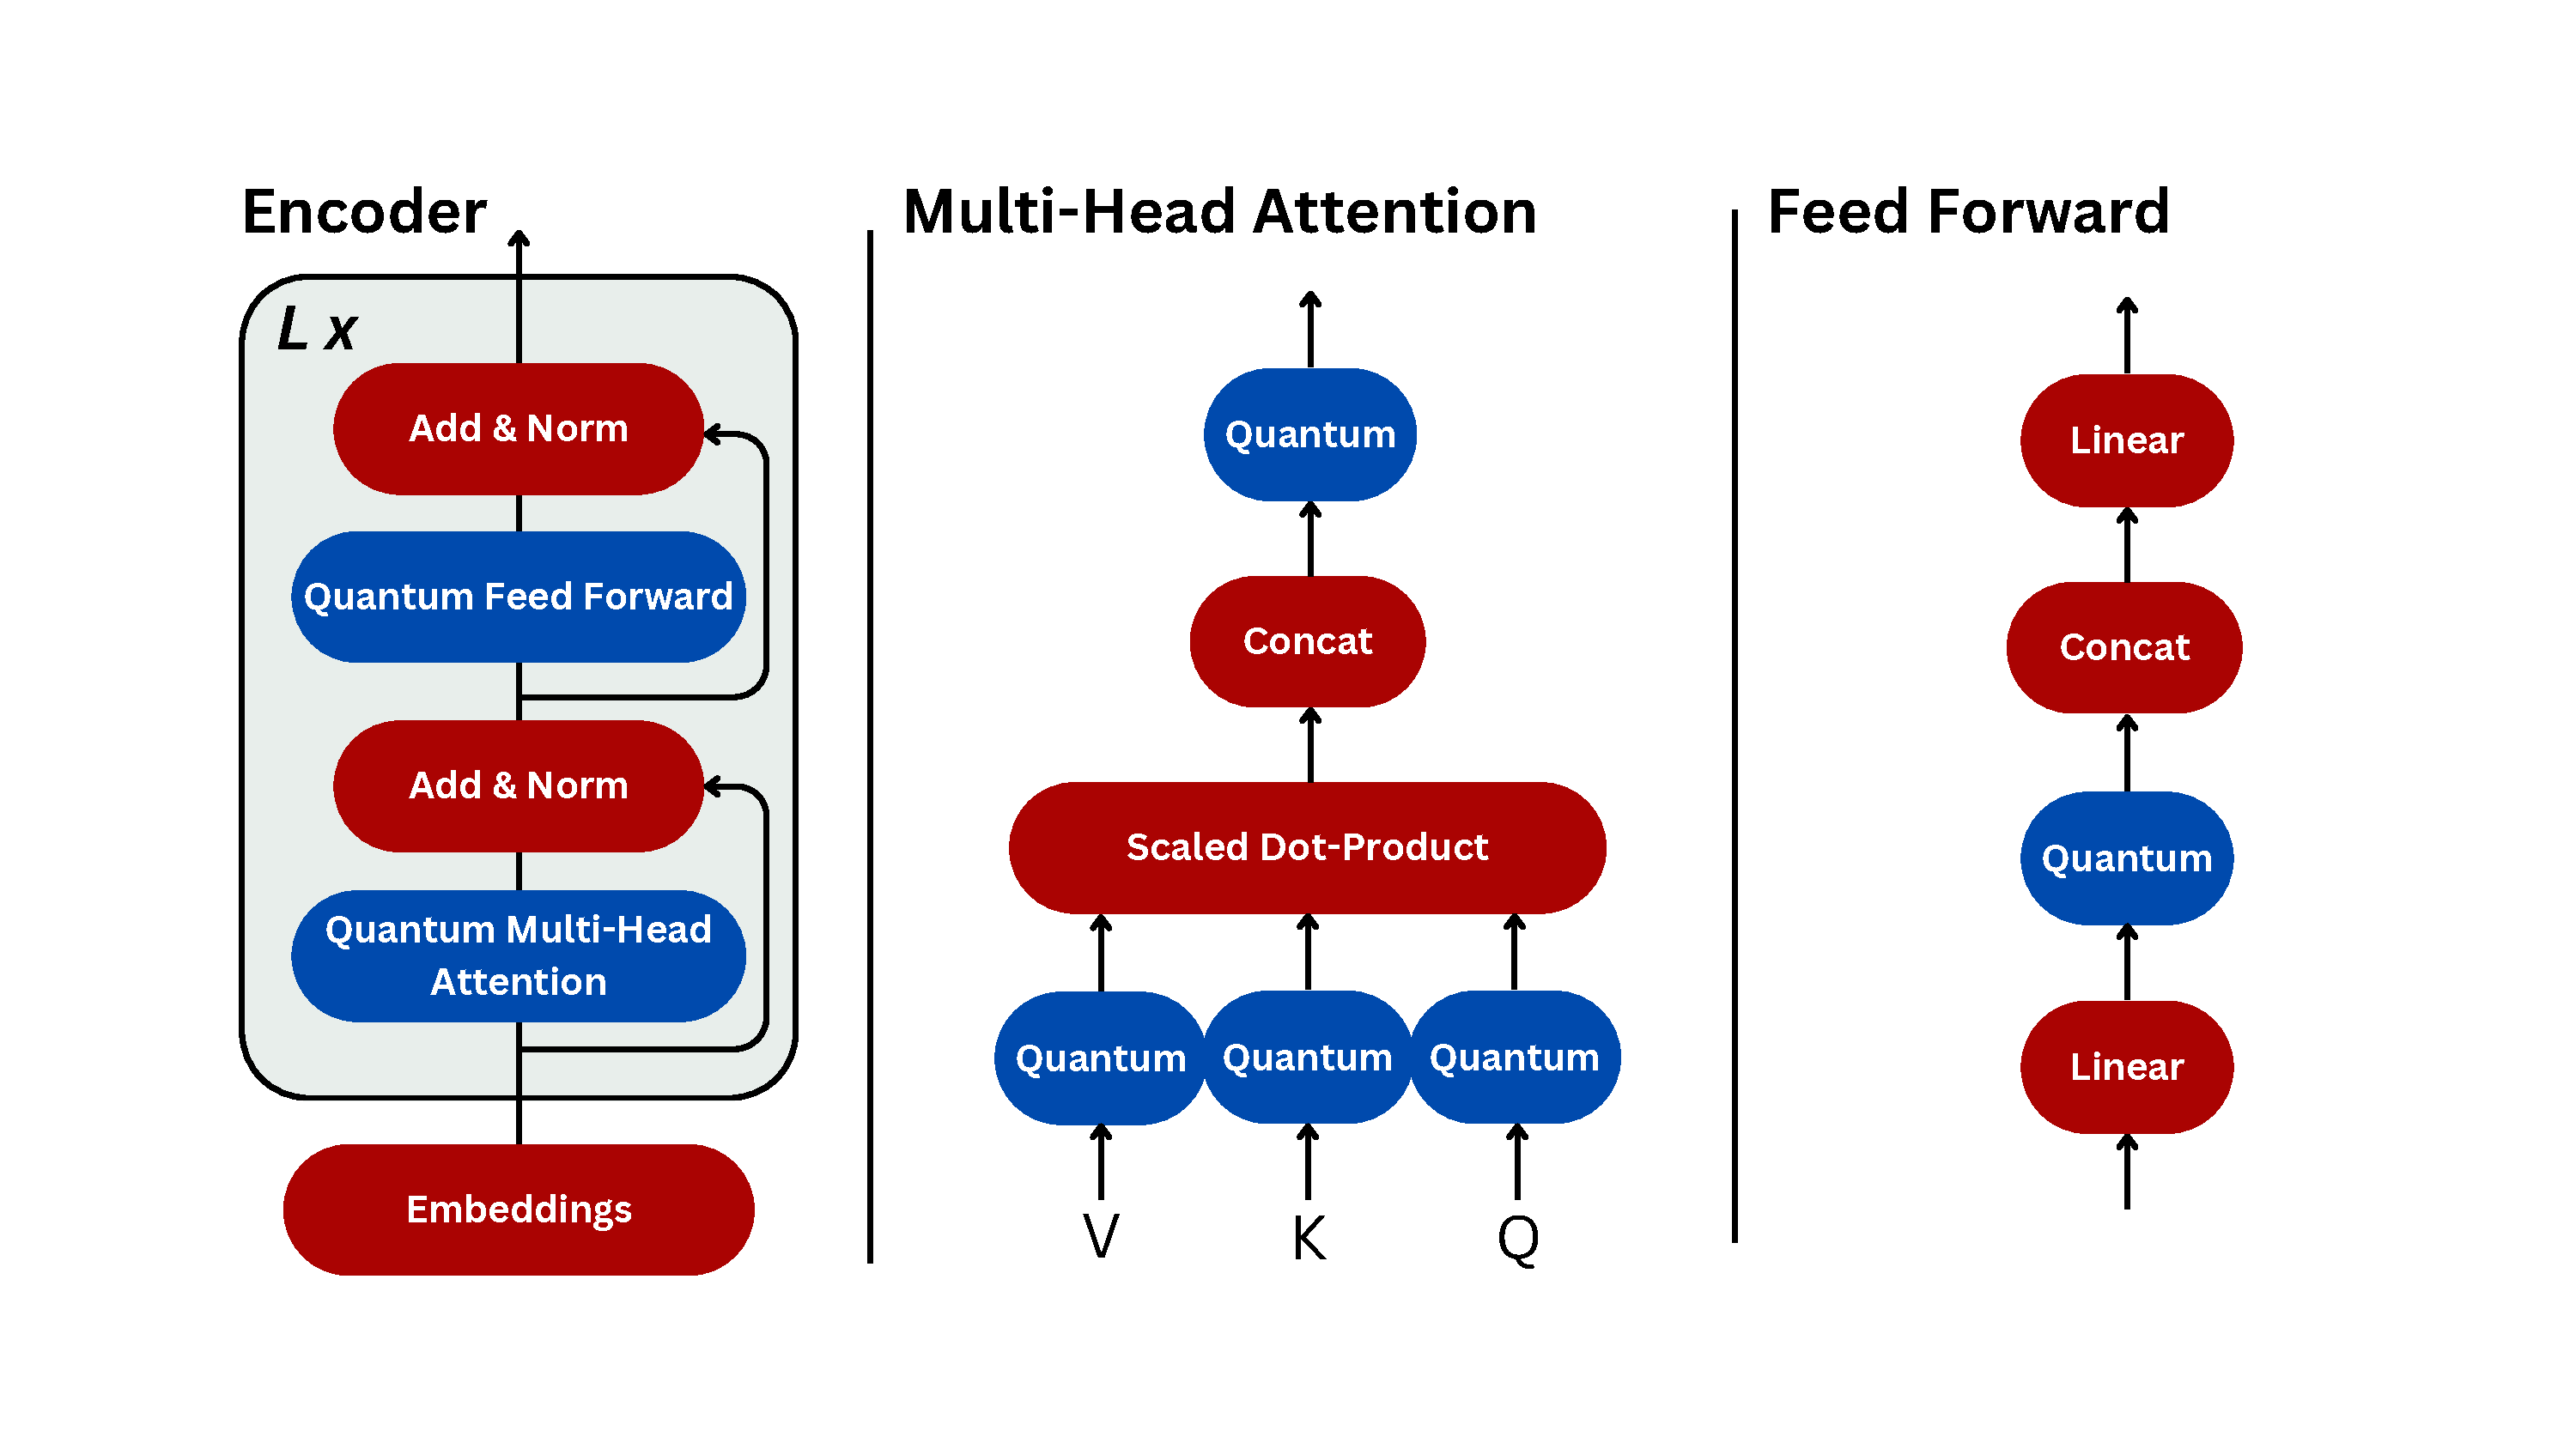
\includegraphics[width=0.98\textwidth]{img/quantum_transformer.pdf}
    }
  \end{center}
  \vspace{-0.5cm}
  \caption{An overview of the quantum transformer. The red components
    represent classical elements, including the embeddings, linear
    layers, and parts of the feedforward and attention mechanisms.
    The blue components denote quantum circuits, where quantum
    multi-head attention and quantum feedforward layers are
    integrated. Specifically, the classical linear layers are
    replaced by \gls{VQC}, which process the word embeddings within
    the quantum sections of the model. The
    illustration of the Transformer Encoder was inspired
    by~\citet{disipio2021dawn}.}
  \label{fig:qt_architecture}
\end{figure}

For the quantum transformer, the classical linear layers were
replaced by \glspl{VQC}, as illustrated in
Figure~\ref{fig:qt_architecture}. These circuits were constructed
using the Pennylane framework. The quantum circuits processed the
word embeddings, with an encoder used to adjust the dimensionality of
the embeddings to match the input size constraints of the quantum
circuits. Various encoding methods, including amplitude encoding and
angle encoding, were employed to translate classical data into
quantum states. For models using amplitude encoding, which compresses
\(2^n\) features down to \(n\) features, a decoder was needed to
decompress the features for the next layer. The basic \gls{VQC}
consisted of a single layer of parameterised gates followed by a ring
of \gls{CNOT} gates, introducing entanglement between qubits. The
strong \gls{VQC} increased the complexity, incorporating three layers
of parameterised gates followed by a ring of \gls{CNOT} gates. This
layering enhanced the expressibility of the model, allowing it to
capture more complex relationships in the input data.

There are also configurations that can be set within the quantum
circuits. For angle encoding, the rotation gate can be chosen from
\(R_x\), \(R_y\), and \(R_z\), depending on the desired rotation
axis. The basic and strong \glspl{VQC} are templates provided by
Pennylane. In the case of the basic VQC, the parameterised rotation
gates can be selected as \(R_x\), \(R_y\), or \(R_z\), giving
flexibility in the choice of rotational operations. However, for the
strong VQC, the parameterised gates are fixed to a sequence of
\(R_z\), \(R_y\), and \(R_z\) gates, which cannot be altered. The
only adjustable component in the strong VQC is the choice of the
two-qubit control gate, where options such as \gls{CNOT}, CZ,
or other controlled gates can be applied.

Finally, the expectation values of the Pauli-Z for all qubits are measured.
Measuring in Pauli-Z corresponds to measuring in the
computational basis (i.e., \( \ket{0} \) and \( \ket{1} \)), which
allows us to interpret the results classically. Although other
measurements, such as Pauli-X, are possible, which measure in the \(
\ket{+} \) and \( \ket{-} \) basis, we focus on Pauli-Z measurements
as they directly reflect the classical binary outcomes needed for
further processing in the model.

Both models were trained and evaluated on identical datasets, with
the same training configurations, including learning rates and batch
sizes. The evaluation focused on comparing the performance of the models
using accuracy metrics. By using the
same datasets and training conditions, the study provided a fair
comparison between the classical and quantum transformer models.
Simulated quantum environments were employed for the quantum model
experiments, using Pennylane and TensorCircuit to run
simulations on classical hardware.

\section{Setup}
\label{sec:setup}
The experiments were conducted in a \gls{HPC} environment using two
types of GPU clusters, depending on the availability of the clusters,
to train and evaluate both classical and quantum transformer models.
The following describes the computational environment:

\begin{itemize}
  \item \textbf{Hardware}: Two different types of GPU nodes were
        utilised from \gls{UWA} cluster:
        \begin{itemize}
          \item \textbf{Large GPU Nodes}: Dual Intel Xeon CPUs (36 cores
                total @ 3.1GHz), 768GB RAM, and Dual NVIDIA 32GB V100 GPU cards.
          \item \textbf{Medium GPU Nodes}: Dual Xeon CPUs (28 cores @
                2.0GHz), 256GB RAM, and 4 NVIDIA 16GB P100 GPU cards.
        \end{itemize}
  \item Only one GPU was used per experiment. This limitation was
        necessary due to Pennylane's own parallelisation mechanisms,
        which are unstable and prone to conflicts with PyTorch’s parallelisation.
        Both GPU nodes were configured to use CUDA 12.4.

  \item \textbf{Software Stack}: The following software stack was used
        for model development and experimentation:
        \begin{itemize}
          \item \textbf{Python}: Python 3.11.8 was used as the core
                language for model development and experimentation.
          \item \textbf{Jupyter Notebook}: All experiments were conducted
                and documented using Jupyter Notebooks for interactive model
                training and evaluation.
          \item \textbf{Conda}: Conda was used as the package manager for
                creating isolated environments with the necessary
                dependencies for both classical (PyTorch, TensorFlow) and
                quantum (Pennylane, TensorCircuit) frameworks.
        \end{itemize}
\end{itemize}

To ensure that all experiments were reproducible, several measures
were implemented. First, all models were seeded, ensuring that the
same random initialisations and conditions were applied across
different experiments. This enabled reproducibility when using the
same hardware and software configurations, ensuring consistency in
the behaviour of the model.

Additionally, intermediate results, such as model checkpoints and
partial outputs, were saved at various stages throughout the training
process. This approach allowed for consistent tracking of progress
and made it easier to reproduce experiments if needed. Saving
intermediate outputs also helped resume training from checkpoints
without having to restart from the beginning.

Lastly, Conda was used to manage the computational environment,
ensuring that dependencies remained consistent across experiments. By
isolating environments, potential issues related to version conflicts
or software updates were avoided, maintaining a stable environment
for the duration of the project.


\chapter{Experiments and Results}
\label{chap:results}
\section{Setup}
\label{sec:setup}
The experiments were conducted within a high-performance computing
environment to facilitate both classical and quantum transformer
model training and evaluation. The following describes the computational setup:

\begin{enumerate}
  \item \textbf{Computational Environment}
        \begin{itemize}
          \item \textbf{Hardware}: All experiments were performed on
                UWA’s \textit{Kaya High-Performance Computing (HPC)} cluster.
                The HPC environment was equipped with NVIDIA GPUs, utilised
                to accelerate the training process for classical models and
                simulate quantum circuits.
          \item \textbf{Quantum Simulators}: For quantum-related
                experiments, we employed quantum simulators available in
                \textit{Pennylane} and \textit{TensorCircuit}. These
                frameworks were used to simulate quantum circuits in the
                absence of physical quantum hardware, allowing for
                experiments involving quantum gate-based computations.
          \item \textbf{Deep Learning Frameworks}: The classical
                transformer models were implemented using \textit{PyTorch}
                and \textit{TensorFlow}, leveraging GPU acceleration where applicable.
        \end{itemize}
\end{enumerate}

\section{Experiments}
\label{sec:experiments}

\section{Results}
\label{sec:results}

\section{Analysis}
\label{sec:analysis}


\chapter{Conclusion and Future Work}
\label{chap:conclusion}
\section{Summary of Contributions}

\section{Future Work}


\appendix
\cftaddtitleline{toc}{chapter}{Appendix}{}
\chapter{Research Proposal}
\label{apx:proposal}
\section{Background}
\label{sec:proposal_background}
The advent of deep learning has been transformative, marking a
paradigm shift in our approach to artificial intelligence. Prior to
2011-2012, deep learning was largely deemed impractical. This
perception changed dramatically when a team participating in the
ImageNet Large Scale Visual Recognition Challenge (ILSVRC) in 2012
leveraged deep learning to secure a dominating lead, outperforming
the second-place team by 9.8 percentage points—a margin that
highlighted the difference between second and third place of 0.8.

The roots of deep learning extend back to 1943, yet it remained
largely theoretical until recent advancements in hardware made its
practical application feasible. Today, we stand on the shoulders of
giants, benefiting from the perseverance of researchers who continued
to explore this field despite its challenges.

Quantum computing holds similar transformative potential. The
transformer model represents the next evolutionary step in deep
learning, and by laying the groundwork for a quantum transformer, we
can pave the way for future advancements.

\citet{disipio2021dawn} proposed a quantum-enhanced transformer for
sentiment analysis by adapting the multi-head self-attention and
feed-forward layers to the quantum realm while~\citet{li2023quantum}
introduced Gaussian Projected Quantum Self-Attention, which they used
to create a Quantum Self-Attention Neural Network for text
classification. They argued that this method is more suitable for
handling quantum data than the straightforward inner-product
self-attention used in the work by~\citet{disipio2021dawn}. Notably,
in both models, the computation of attention coefficients and outputs
remains within the classical domain.

In terms of performance,~\citet{Cherrat_2024} provided results
supporting the notion that quantum transformers may match the
performance of their classical counterparts while requiring fewer
resources in terms of runtime and parameter count. However, their
approach has faced criticism, particularly regarding the exponential
cost associated with encoding matrices into quantum states.

The field of quantum computing is poised to revolutionise deep
learning, yet the integration of quantum mechanisms within neural
network architectures remains under-explored. This study seeks to
address the problem of how quantum components, specifically
variational quantum circuits, can be effectively incorporated into
transformer models to enhance their learning efficiency and reduce
generalisation errors. Specifically, we seek to enhance the
quantum-enhanced transformer initially proposed
by~\citet{disipio2021dawn}. We hypothesise that a quantum transformer
will require less training time and exhibit improved performance
metrics compared to its classical counterparts.

\section{Aim}
\label{sec:aim}
To develop and validate a quantum transformer model that integrates
variational quantum circuits into its architecture, thereby enhancing
learning efficiency and reducing generalisation errors. This will involve:

\begin{enumerate}
    \setlength{
  \itemsep}{-1ex}
  \item Analysing the current limitations of classical transformer
    models in terms of learning efficiency and generalisation.
  \item Designing a quantum transformer architecture that
    incorporates variational quantum circuits as a core component.
  \item Comparing the performance of the proposed quantum transformer
    with classical models, focusing on training time and performance metrics.
  \item Assessing the feasibility of the quantum transformer in
    practical applications, considering both its computational
    efficiency and the quality of its outputs.
\end{enumerate}

\section{Methodology}
\label{sec:methodology}
\subsection{Data Collection}
\label{subsec:data_collection}

Before diving into our models, it is essential to outline the
datasets employed in this study. We start with a lightweight dataset,
which lays the groundwork for our initial analysis then transition to
a more sophisticated dataset, presenting a richer set of challenges
and opportunities for our models to tackle.

In this project, we will use three well-known text classification
datasets: the IMDb, Amazon Polarity, and Yelp Reviews Polarity
datasets, to explore the performance of our models.

The IMDb dataset consists of 50,000 movie reviews, making it ideal
for natural language processing and text analytics. This dataset is
designed for binary sentiment classification, where each review is
classified as either positive or negative. With 25,000 movie reviews
allocated for training and another 25,000 for testing, this dataset
offers a robust amount of data for sentiment analysis tasks. Our
model will predict the polarity of reviews, aiming to differentiate
between positive and negative sentiments using deep learning or
classification algorithms.

The Amazon Polarity dataset is a collection of product reviews
sourced from Amazon over an 18-year period. The dataset includes
approximately 35 million reviews up to March 2013. Reviews with
ratings of 1 and 2 are labelled as negative (class 1), while reviews
rated 4 and 5 are labelled as positive (class 2), with reviews rated
3 being excluded. The dataset provides 1,800,000 training samples and
200,000 testing samples for each class, making it a large-scale
dataset well-suited for binary classification tasks. The inclusion of
product and user information, ratings, and plaintext reviews enables
us to further explore consumer sentiment through our text transformer.

The Yelp Reviews Polarity dataset is derived from the 2015 Yelp
Dataset Challenge and consists of 1,569,264 samples of review text.
For this polarity classification task, reviews with star ratings of 1
and 2 are labelled as negative, while reviews rated 3 and 4 are
labelled as positive. The dataset provides 280,000 training samples
and 19,000 test samples per polarity class. This dataset provides
another large and diverse set of review data that can be utilised to
refine our text transformer model, further strengthening its ability
to classify sentiment in various domains.

\subsection{Models}
\label{subsec:models}

\subsubsection{Classical Transformer}
\label{subsubsec:classical_vision_transformer}

We will implement a classical transformer based on the standard
architecture as shown in Figure~\ref{fig:vit_architecture}. While the
diagram represents the structure of a vision
transformer, the overall structure of the text transformer will be
similar, with key modifications to accommodate text-based input. We
chose the standard transformer encoder model to serve as the baseline
for our benchmark. The general steps of our text transformer are as follows:

\begin{enumerate}
    \setlength{
  \itemsep}{-1ex}
  \item The input text is tokenised into sequences of words or
    subwords using a pre-trained tokenizer.
  \item Each token is then transformed into embeddings using a
    pre-trained word embedding model such as BERT.
  \item Since the transformer processes the tokens in parallel, it
    does not inherently capture the order of the sequence. To address
    this, positional embeddings are added to the token embeddings to
    encode the sequential information.
  \item The new embeddings, along with an additional special token
    embedding, are passed through the transformer encoder.
  \item The output of the encoder is then processed by a multi-layer
    perceptron (MLP) head, which converts the token representations
    into a class prediction for sentiment analysis.
\end{enumerate}

\begin{figure}[ht]
  \begin{center} \subfloat[Vision Transformer Architecture]{
    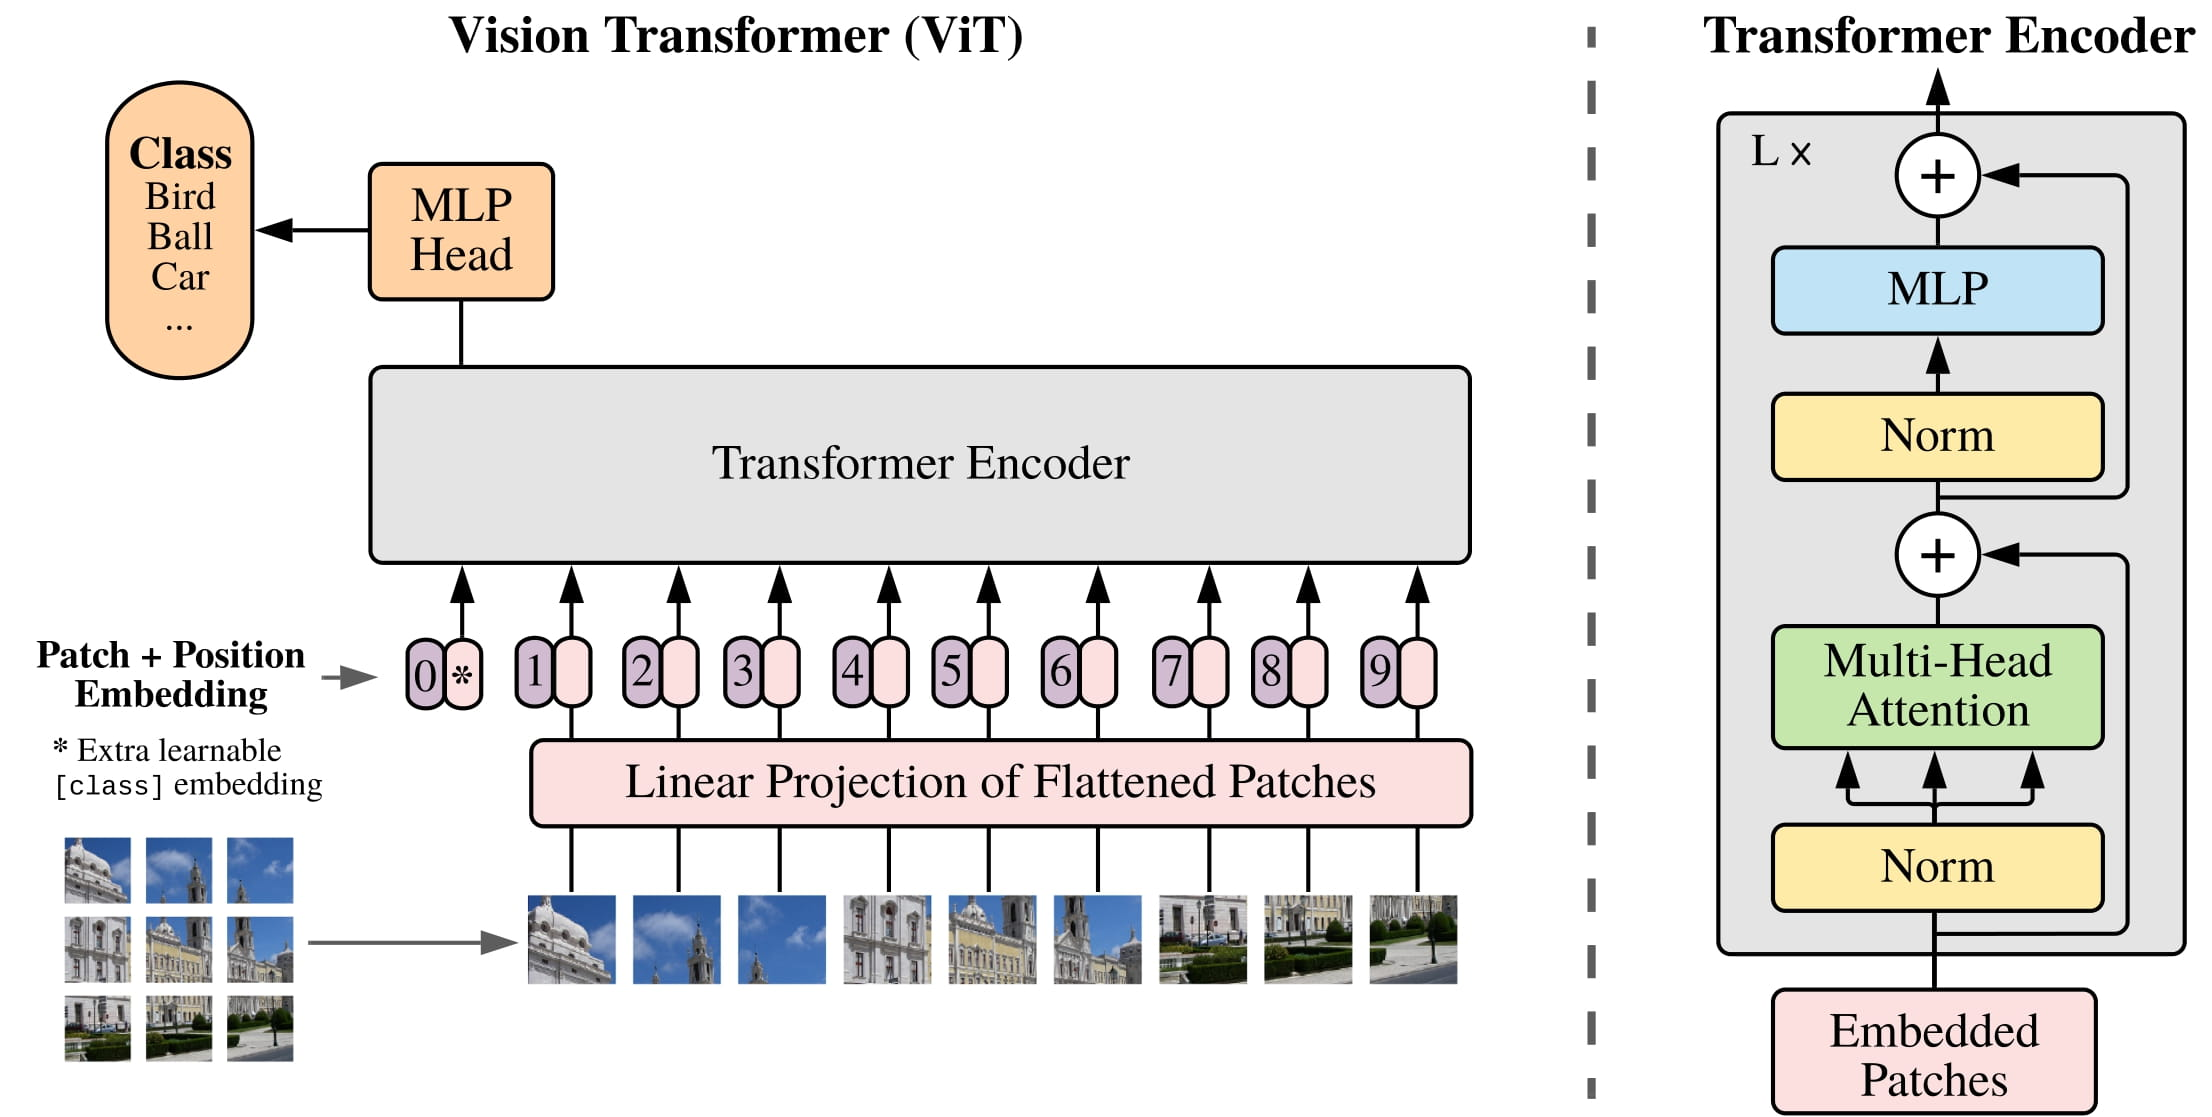
\includegraphics[height=0.4\textwidth]{img/vit_architecture.jpg} }
  \end{center} \vspace{-0.5cm} \caption{An overview of the classical
  model~\cite{dosovitskiy2021image}.}
  \label{fig:vit_architecture}
\end{figure}

In the standard transformer encoder, we use multi-head attention,
which employs several self-attention mechanisms to capture different
types of relationships between tokens. The multi-layer perceptrons
(MLPs) contain two layers with Gaussian Error Linear Unit (GELU)
non-linearity to model complex interactions between tokens. Layer
normalisation stabilises and accelerates training, while residual
connections prevent the vanishing gradient problem.

This architecture will be adapted to text-based sentiment analysis
tasks using datasets such as IMDb, Amazon Polarity, and Yelp Reviews Polarity.

\subsubsection{Quantum Transformer}
\label{subsubsec:quantum_vision_transformer}

\begin{figure}[ht]
  \begin{center}
    \subfloat[Quantum Vision Transformer Architecture]{
      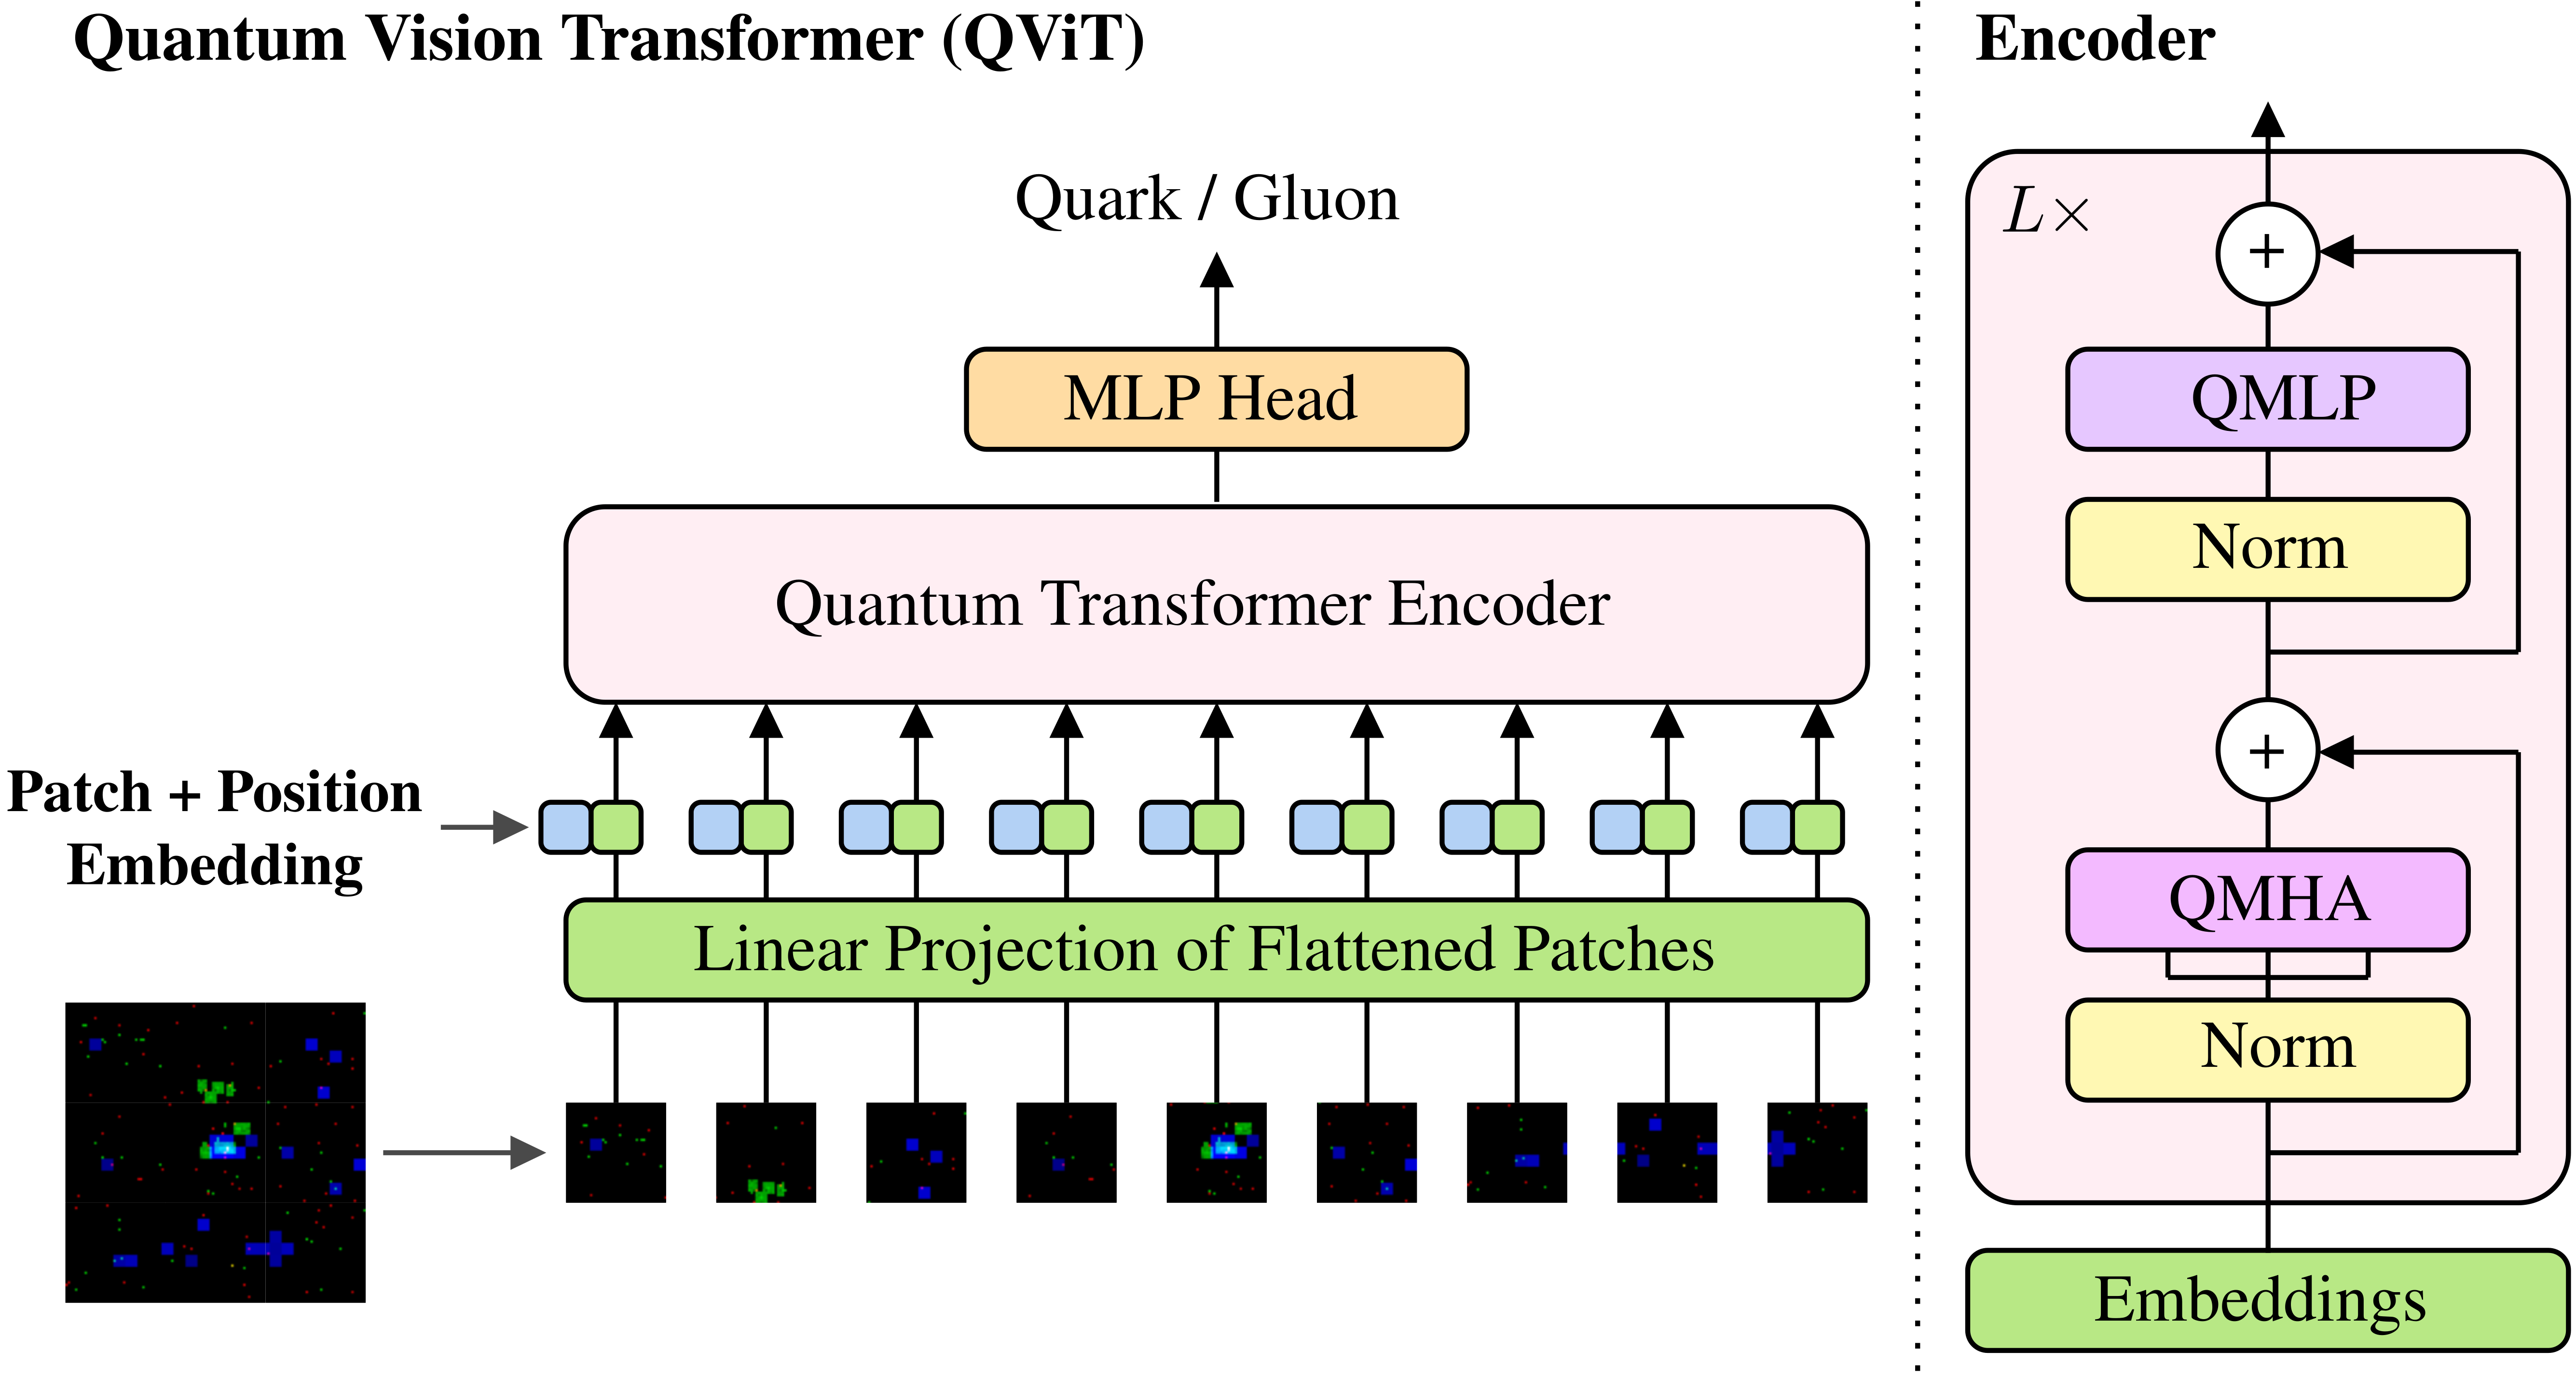
\includegraphics[height=0.4\textwidth]{img/qvit_architecture.png}
    }
  \end{center}
  \vspace{-0.5cm}
  \caption{An overview of the quantum model~\cite{Cara_2023}. The
    illustration of the Transformer Encoder was inspired
  by~\citet{disipio2021dawn}.}
  \label{fig:qvit_architecture}
\end{figure}

\citet{Cara_2023} introduced a model depicted in
Figure~\ref{fig:qvit_architecture}, which incorporates variational
quantum circuits into the multi-head attention and multi-layer
perceptron components of the original architecture. These circuits
serve as the equivalent of fully-connected layers within both
components, potentially offering improved performance in specific
tasks. As our comprehension of the quantum transformer
deepens, the model may be further augmented with additional quantum components.

\subsection{Training and Evaluation}
\label{subsec:training_and_evaluation}

To maintain consistency with the previous work by \citet{Cara_2023}
and \citet{Cherrat_2024}, we will adopt similar hyper-parameters:
cross-entropy loss function, Adam optimizer, 100 training epochs, a
batch size of 32 and a learning rate of \(10^{-3}\).

For model performance evaluation, we will employ two metrics: the
area under the receiver operating characteristic (ROC) curve (AUC)
and accuracy (ACC).

\section{Software and Hardware Requirements}
\label{sec:requirements}

\subsection{Software}
\label{subsec:software}
\begin{itemize}
    \setlength{
  \itemsep}{-1ex}
  \item Python: An easy-to-learn and really popular programming
    language to write quantum code.
  \item PyTorch: A Python library for deep learning.
  \item TensorFlow: Another Python library for deep learning.
  \item PennyLane: A Python library for quantum machine learning.
  \item TensorCircuit: Another Python library for quantum machine learning.
  \item Overleaf: An online latex editor for documentation.
  \item GitHub: An online hub to version control the code for this project.
  \item Visual Studio Code: A code editor to write Python code and
    SSH into Kaya.
  \item Hugging Face: A machine learning platform for sharing machine
    learning models and datasets.
\end{itemize}

\subsection{Hardware}
\label{subsec:hardware}

\begin{itemize}
    \setlength{
  \itemsep}{-1ex}
  \item Personal Laptop: A device to write and edit code.
  \item Kaya: The UWA High-Performance Computational Research Platform.
\end{itemize}

\section{Timeline}
\label{sec:timeline}
The following comprises a rough timeline for the outlined project.

\begin{itemize}
    \setlength{
  \itemsep}{-1ex}
  \item Research proposal: 18th of March
  \item Quantum Computing Study: February - 14 October
    \begin{itemize}
        \setlength{
      \itemsep}{-1ex}
      \item Textbook Readings:
        \begin{itemize}
          \item Explorations in Quantum Computing (Recommended by Jingbo)
          \item Quantum Computing for Computer Scientists
            (Recommended by Microsoft)
          \item Quantum Computation and Quantum Information
            (Recommended in the Quantum Computing Subreddit)
        \end{itemize}
      \item Interactive Learning:
        \begin{itemize}
          \item IBM Quantum
          \item Microsoft Azure Quantum
          \item PennyLane Xanadu Quantum Codebook
        \end{itemize}
    \end{itemize}
  \item Implement a classical transformer from scratch: 18 March - 31 March
  \item Train and evaluate the transformer: April - May
  \item Literature Review: March - 13 May
  \item Implement a quantum transformer: May - August
  \item Seminar Abstract: August - 16 September
  \item Seminar: August - (30 September - 4 October)
  \item Thesis: August - 14 October
\end{itemize}


\chapter{Pseudo Code}

\chapter{Training Speed Analysis}

\chapter{User Manual}


\chapter*{Bibliography}
\label{bibliography}
\addcontentsline{toc}{chapter}{Bibliography}
\bibliographystyle{abbrvnat}
\setlength{\bibsep}{2pt}
\let\oldaddcontentsline\addcontentsline% Store \addcontentsline
\renewcommand{\addcontentsline}[3]{}% Make \addcontentsline a no-op
\renewcommand{\bibname}{}
\bibliography{3_footer/references.bib}
\let\addcontentsline\oldaddcontentsline% Restore \addcontentsline

\end{document}
